\documentclass[11pt]{article}

\usepackage[margin=1in]{geometry}
\usepackage[T1]{fontenc}
\usepackage{lmodern}
\usepackage{microtype}
\usepackage{setspace}
\usepackage{booktabs}
\usepackage{graphicx}
\usepackage{amsmath}
\usepackage{caption}
\usepackage[hidelinks]{hyperref}

\onehalfspacing
\captionsetup{font=small, labelfont=bf}
\graphicspath{{../output/figures/}}

% Video identifiers as they appear in the data.
\newcommand{\vid}[1]{\texttt{#1}}
\newcommand{\tablenote}[1]{\par\vspace{4pt}\begin{minipage}{\linewidth}\footnotesize #1\end{minipage}}

\title{Which Messages Persuade? Unbundling the Effects of Chinese State Media\\[4pt]
\large A Replication and Extension of Mattingly et al.\ (2025)}
\author{Yuxuan Zhang\\ \small Harris School of Public Policy, University of Chicago}
\date{October 2026}

\begin{document}

\maketitle

\begin{abstract}
\noindent Mattingly et al.\ (2025) show in a 19-country experiment that short videos from China's state broadcaster CGTN substantially increase preference for China's political and economic models over those of the United States. I reproduce the paper's main results in Python from the authors' replication data; every coefficient, standard error, and sample size in the primary results table matches the published values. I then extend the analysis by exploiting a second layer of randomization that the paper does not analyze: within treatment arms, the specific videos each respondent saw were also randomly assigned. Two findings emerge. First, within the China arm, an economic rather than a second political video raises preference for China's economic model by 0.26 points on a six-point scale but has no detectable effect on preference for its political model. Second, in the arm where Chinese and US videos compete head-to-head, the four CGTN videos differ markedly in persuasiveness, and the least persuasive one is the video that every respondent in the China arm saw. Both findings suggest that the persuasive power of state media depends on the specific message, and that the paper's China-arm estimate may be conservative relative to other combinations of CGTN content.
\end{abstract}

\section{Introduction}

Can an authoritarian state persuade foreign publics that its model of governance is superior? Mattingly, Incerti, Ju, Moreshead, Tanaka, and Yamagishi (2025) answer this question with a large preregistered experiment. In June 2022, they showed 6,276 respondents in 19 countries short videos produced by China's state broadcaster CGTN, by the US State Department, by both, or neither, and then asked whether they preferred the Chinese or the American political and economic model. The effects are large. Two CGTN videos raise the share of respondents preferring China's political model from 16 to 54 percent. US videos move respondents toward the American model, but by less. And when respondents see one video from each country, opinion still shifts toward China.

Each treatment in the experiment is a \emph{bundle} of two videos, and the paper estimates the effect of each bundle as a whole. In their conclusion, the authors identify unbundling the treatments as a priority for future research: which specific messages are most persuasive, and why? This paper takes a first step in that direction using the original data.

The paper makes two contributions. The first is a replication. I re-implement the authors' primary analysis in Python, starting from their analysis dataset, and reproduce all sixteen coefficients and standard errors in their primary results table exactly at the reported precision. Along the way I document how the analysis sample is constructed and several details that matter when moving the analysis from R to Python.

The second contribution is an extension. The experiment randomized not only which arm a respondent entered but also which videos they saw within it. I show that this within-arm randomization has a specific structure. In the China and US arms, every respondent saw the same political video, and only the companion video was randomized. In the Competition arm, the Chinese and US videos were drawn independently, forming a four-by-four factorial design. Because these assignments are random, comparisons across videos within an arm are as credibly causal as the paper's comparisons across arms. I use them to estimate the effect of economic versus political content and the effect of each individual video.

The results point in a consistent direction. Message content matters, but mostly within its own domain: CGTN's economic videos raise preference for China's economic model without adding anything to preference for its political model beyond what a second political video provides. Individual videos also differ substantially in persuasiveness, and these differences do not reduce to the economic-versus-political distinction. Because the weakest CGTN video in the Competition arm was shown to every respondent in the China arm, the paper's headline China-arm effect may understate what other combinations of CGTN content could achieve. All of these comparisons rely on a small number of videos and smaller subsamples, so I report minimum detectable effects and multiple-comparison-adjusted $p$-values throughout and interpret null results cautiously.

\section{The Original Study}

\paragraph{Argument.} Mattingly et al.\ (2025) argue that audiences evaluate political systems not only on democratic values but also on government performance: economic growth, stability, competent leadership, and responsiveness. Chinese state media emphasize exactly these dimensions. A second part of the argument concerns prior beliefs. Foreign audiences typically know much more about the United States than about China, so their beliefs about China are weaker and more easily moved by new information.

\paragraph{Design.} The experiment was fielded on Lucid between June 10 and 19, 2022, in 19 English-, Spanish-, and Arabic-speaking countries across Africa, Asia, Europe, North America, Oceania, Latin America, and the Middle East. Respondents had to pass two pre-treatment attention checks. They were then randomly assigned, within country, with equal probability to one of four arms:
\begin{itemize}\setlength\itemsep{0pt}
  \item \textbf{Control}: two nature videos;
  \item \textbf{China}: two of four CGTN videos;
  \item \textbf{USA}: two of four US State Department videos;
  \item \textbf{Competition}: one CGTN video and one US video.
\end{itemize}
Each country's video pool contained two videos promoting its political model and two promoting its economic model. The authors selected these videos from large corpora of CGTN and State Department content which they characterize with topic models, and use text-based distance measures to show that the selected videos are representative of what each broadcaster produces.

\paragraph{Outcomes and estimation.} The primary outcomes are two six-point scales asking whether respondents prefer the US or the Chinese political model and economic model (1 = strongly prefer the United States, 6 = strongly prefer China). The authors estimate effects by OLS with HC2 robust standard errors, both without covariates and with country fixed effects plus gender, age, education, national pride, and left--right ideology. Missing covariate values are imputed by predictive mean matching.

\paragraph{Findings.} All three treatments have large and precisely estimated effects (Table~\ref{tab:replication}). The China treatment raises preference for China's political model by 1.04 points and for its economic model by 0.87 points. The US treatment lowers them by 0.43 and 0.57 points. When the two compete, the net effect still favors China (0.36 and 0.28 points). Mechanism analyses suggest that CGTN videos work mainly by improving perceptions of China's performance rather than of its democratic qualities.

\section{Replication}

\subsection{Data and Sample}

The replication package includes the raw Qualtrics exports, the authors' cleaning script, and the cleaned analysis dataset. I start from the cleaned dataset rather than the raw exports for one reason. The authors impute missing covariates with the R package \texttt{mice}, and the imputed values depend on R's random number generator. They cannot be reproduced exactly in Python, so re-running the imputation would produce small differences in the covariate-adjusted estimates that reflect software rather than substance. I read the authors' cleaning script line by line and confirmed every step that affects the analysis sample.

The cleaned file contains 12,941 respondents, of whom 6,276 were randomized. Table~\ref{tab:flow} shows where the others left the survey. The categories are mutually exclusive and follow the order of the questionnaire. More than two in five respondents who completed the attention checks failed them, so the analysis sample is selected toward attentive respondents. This selection happens before randomization, so it does not threaten the comparison between arms, but it does define the population to which the estimates apply.

\begin{table}[ht]
\centering
\caption{Construction of the analysis sample}
\label{tab:flow}
\begin{tabular}{lr}
\toprule
Stage & Respondents \\
\midrule
Screened out: not a citizen of the survey country & 955 \\
Left before the attention checks & 859 \\
Failed an attention check & 4,830 \\
Passed the checks but left before randomization & 21 \\
\textbf{Randomized} & \textbf{6,276} \\
\midrule
Total in the authors' cleaned dataset & 12,941 \\
\bottomrule
\end{tabular}
\tablenote{\emph{Note:} Respondents who left before randomization have no treatment assignment and no outcome data, so they drop out of every model in the original analysis. The authors' cleaning script also removes a separate Japan experiment and respondents with no country; neither group is in the cleaned file.}
\end{table}

\subsection{Specification}

I estimate, separately for each outcome $Y_i$,
\begin{equation}
Y_i = \alpha + \beta_1\,\text{China}_i + \beta_2\,\text{USA}_i + \beta_3\,\text{Competition}_i + \mathbf{X}_i'\boldsymbol{\gamma} + \varepsilon_i,
\label{eq:main}
\end{equation}
where Control is the omitted category and $\mathbf{X}_i$ contains country fixed effects and the five covariates entered linearly, exactly as in the authors' code. The unadjusted model omits $\mathbf{X}_i$. Standard errors are HC2, the default of the \texttt{estimatr} package the authors use. With only treatment indicators on the right-hand side, HC2 coincides with the conservative Neyman variance estimator for a difference in means (Samii and Aronow 2012).

Three implementation details turned out to matter. First, the Python reader for R data files does not preserve the order of R factor levels: it sorts the treatment arms alphabetically, which would silently make China rather than Control the reference category. I restore the original order explicitly. Second, the country identifier must remain a string. In both R and Python, the reference country for string identifiers is the first in lexical order (code ``10'', Kenya), which determines the constant in the adjusted model. Third, the standard error type must be specified explicitly, because Python's default is not HC2.

\subsection{Results}

Table~\ref{tab:replication} reports the replicated estimates. Every coefficient, standard error, and sample size is identical to the published Table A3 when rounded to two decimals; an automated cell-by-cell comparison is included in the code repository. Figure~\ref{fig:main} displays the covariate-adjusted effects. Adjusting for covariates barely moves the point estimates (for the China arm's effect on the political model, from 1.045 to 1.040) and modestly shrinks the standard errors, as expected when treatment is randomized and covariates are prognostic.

\begin{table}[ht]
\centering
\caption{Replication of the primary results (Mattingly et al.\ 2025, Table A3)}
\label{tab:replication}
\begin{tabular}{lcccc}
\toprule
 & \multicolumn{2}{c}{Covariate-adjusted} & \multicolumn{2}{c}{Unadjusted} \\
\cmidrule(lr){2-3}\cmidrule(lr){4-5}
 & Political & Economic & Political & Economic \\
\midrule
China       & 1.04 (0.05)  & 0.87 (0.05)  & 1.05 (0.05)  & 0.87 (0.06) \\
USA         & $-$0.43 (0.04) & $-$0.57 (0.05) & $-$0.44 (0.04) & $-$0.58 (0.05) \\
Competition & 0.36 (0.05)  & 0.28 (0.06)  & 0.37 (0.05)  & 0.28 (0.06) \\
Constant    & 3.32 (0.20)  & 3.76 (0.23)  & 2.56 (0.03)  & 2.88 (0.04) \\
\midrule
Covariates and country FE & Yes & Yes & No & No \\
$N$         & 5,952 & 5,946 & 5,952 & 5,946 \\
\bottomrule
\end{tabular}
\tablenote{\emph{Note:} OLS estimates with HC2 robust standard errors in parentheses. Outcomes range from 1 (strongly prefer the US model) to 6 (strongly prefer the Chinese model). Covariates are gender, age, education, national pride, and left--right ideology. All entries match the published values at two decimals.}
\end{table}

\begin{figure}[ht]
\centering
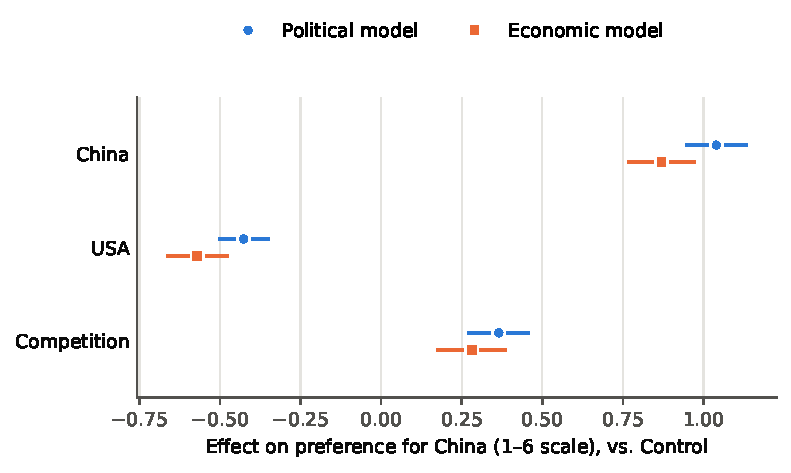
\includegraphics[width=0.8\linewidth]{fig1_main_effects.pdf}
\caption{Covariate-adjusted effects of each treatment arm relative to Control. Points are OLS estimates; lines are 95\% confidence intervals based on HC2 standard errors.}
\label{fig:main}
\end{figure}

To convey magnitude, I follow the authors in dividing the unadjusted effects by the control-group standard deviation of each outcome. The China treatment moves preference for China's political model by 0.87 standard deviations and for its economic model by 0.59, both large by the standards of survey experiments. In raw terms, the share of respondents preferring China's political model rises from 16.3 percent in the control group to 54.3 percent in the China arm.

\section{Extension: Unbundling the Treatments}

\subsection{Motivation}

The replication confirms that a bundle of two CGTN videos is highly persuasive. It does not tell us which content does the work. This question matters both for theory and for policy. If the effect operates through performance information, as the authors argue, then videos about economic achievement might be especially effective, perhaps even for views about the political model. Alternatively, persuasion might depend on idiosyncratic features of particular videos, in which case the effect of ``Chinese state media'' would depend heavily on which messages audiences happen to see.

\subsection{Within-Arm Randomization}

The data record the identifiers of the two videos each respondent saw. Cross-tabulating them reveals the structure of the within-arm randomization, which is not fully described in the paper.

\paragraph{China and USA arms.} Every respondent in the China arm saw the same political video, \vid{china\_pol2}, and every respondent in the USA arm saw \vid{us\_pol2}. Only the second, \emph{companion} video was randomized: about half of respondents saw the other political video (\vid{pol1}), and about a quarter each saw one of the two economic videos (Table~\ref{tab:companion_n}). Holding \vid{pol2} fixed, comparing respondents whose companion was economic with those whose companion was political therefore estimates the causal effect of substituting economic for political content in the second slot. The cost is that the separate effect of \vid{pol2} cannot be identified in these arms, since no one in them was shown a different pair without it.

\begin{table}[ht]
\centering
\caption{Video combinations in the China arm}
\label{tab:companion_n}
\begin{tabular}{llr}
\toprule
Companion video (randomized) & Always shown & Respondents \\
\midrule
\vid{china\_pol1} & \vid{china\_pol2} & 778 \\
\vid{china\_econ1} & \vid{china\_pol2} & 415 \\
\vid{china\_econ2} & \vid{china\_pol2} & 429 \\
\bottomrule
\end{tabular}
\tablenote{\emph{Note:} The USA arm has the same structure, with \vid{us\_pol2} always shown (771, 411, and 383 respondents). The replication package does not include the survey flow file, so I cannot confirm from the instrument itself whether \vid{pol2} was always shown by design or whether the stored labels were reassigned; the data are consistent with the former.}
\end{table}

\paragraph{Competition arm.} Here one US video and one Chinese video were each drawn from all four of the country's videos, independently of each other. All sixteen combinations occur, each with 79 to 107 respondents. A chi-squared test does not reject independence of the two assignments ($\chi^2 = 10.42$, $df = 9$, $p = 0.32$). This four-by-four factorial identifies the effect of each Chinese video relative to the others while the US video is balanced by randomization, and vice versa.

The paper reports that the order of the two videos in the Competition arm was randomized. I had planned to study order effects, but the stored video variables are organized by country rather than by display order (the first always records the US video), and the raw survey exports contain no display-order field. Order effects therefore cannot be studied with the public data.

\subsection{Estimation}

For the China and USA arms, I estimate within each arm
\begin{equation}
Y_i = \alpha + \delta\,\text{EconCompanion}_i + \mathbf{X}_i'\boldsymbol{\gamma} + \varepsilon_i,
\label{eq:companion}
\end{equation}
where $\delta$ is the effect of an economic rather than political companion video. For the Competition arm, I estimate
\begin{equation}
Y_i = \alpha + \theta_C\,\text{ChinaEcon}_i + \theta_U\,\text{USEcon}_i + \mathbf{X}_i'\boldsymbol{\gamma} + \varepsilon_i,
\label{eq:types}
\end{equation}
both as written and with an interaction between the two indicators. I also replace the two type indicators with indicators for each specific video, using \vid{pol2} as the reference for each country because it is the video held fixed in the single-country arms. All models use the same covariates and HC2 standard errors as the replication. Within each family of tests I report $p$-values adjusted by the Holm (1979) and Benjamini--Hochberg (1995) procedures, which the authors also use. For the single-country comparisons I report the minimum detectable effect (MDE) at 80 percent power and a two-sided 5 percent test, $\text{MDE} = (z_{0.975} + z_{0.80}) \times \text{SE} \approx 2.8 \times \text{SE}$.

\subsection{Results: Economic versus Political Content}

Table~\ref{tab:companion} and Figure~\ref{fig:companion} report the companion-video comparisons. In the China arm, replacing a second political video with an economic one raises preference for China's economic model by 0.26 points (SE 0.08; Holm-adjusted $p = 0.004$), nearly a third of the full China-arm effect on that outcome. The same substitution has no effect on preference for China's political model: the estimate is 0.01 (SE 0.08), with a confidence interval from $-0.14$ to $0.16$. Given an MDE of 0.21, the data rule out large differences, though not modest ones.

In the USA arm, neither difference is distinguishable from zero. The US economic and political videos move opinion by similar amounts when shown on their own.

\begin{table}[ht]
\centering
\caption{Effect of an economic rather than political companion video}
\label{tab:companion}
\begin{tabular}{llcccccc}
\toprule
Arm & Outcome & Estimate & SE & Holm $p$ & BH $p$ & MDE & $N$ \\
\midrule
China & Political model & 0.009 & 0.076 & 1.000 & 0.905 & 0.214 & 1,527 \\
China & Economic model  & 0.256 & 0.077 & 0.004 & 0.004 & 0.216 & 1,526 \\
USA   & Political model & 0.076 & 0.053 & 0.456 & 0.304 & 0.149 & 1,489 \\
USA   & Economic model  & 0.011 & 0.065 & 1.000 & 0.905 & 0.182 & 1,487 \\
\bottomrule
\end{tabular}
\tablenote{\emph{Note:} Each row is a separate OLS regression within one arm (Equation~\ref{eq:companion}), with country fixed effects, covariates, and HC2 standard errors. Positive values mean more favorable to China. $p$-values are adjusted across the four tests. MDE: minimum detectable effect at 80\% power, $\alpha = 0.05$.}
\end{table}

\begin{figure}[ht]
\centering
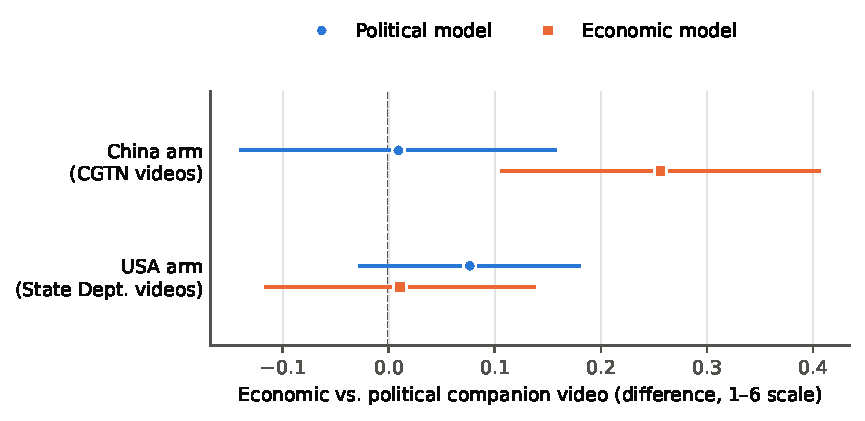
\includegraphics[width=0.8\linewidth]{fig2_companion.pdf}
\caption{Effect of an economic rather than political companion video within the China and USA arms. Points are OLS estimates; lines are unadjusted 95\% confidence intervals.}
\label{fig:companion}
\end{figure}

The pattern for CGTN suggests that content persuades mainly within its own domain. Economic videos improve views of China's economic model, but they do not spill over to its political model more than a second political video does. Neither do they do worse: for the political outcome, the two types of content appear to be close substitutes.

\subsection{Results: Individual Videos in Competition}

Table~\ref{tab:types} reports the type-level estimates from the Competition arm. A Chinese economic video, compared with a Chinese political one, raises preference for China's political model by 0.28 points and for its economic model by 0.56 points; both survive the Holm correction. On the US side, economic and political videos have the same effect on the political outcome, but a US economic video pulls respondents 0.24 points further toward the US economic model. The interaction terms are negative but imprecise and not significant.

\begin{table}[ht]
\centering
\caption{Effects of video type in the Competition arm}
\label{tab:types}
\begin{tabular}{lcccc}
\toprule
 & \multicolumn{2}{c}{Political model} & \multicolumn{2}{c}{Economic model} \\
\cmidrule(lr){2-3}\cmidrule(lr){4-5}
 & Estimate (SE) & Holm $p$ & Estimate (SE) & Holm $p$ \\
\midrule
\multicolumn{5}{l}{\emph{Additive model}} \\
Chinese video is economic & 0.282 (0.078) & 0.001 & 0.560 (0.082) & $<$0.001 \\
US video is economic      & 0.023 (0.077) & 0.767 & $-$0.235 (0.082) & 0.008 \\
\midrule
\multicolumn{5}{l}{\emph{Interaction model}} \\
Chinese econ.\ $\times$ US econ. & $-$0.178 (0.155) & --- & $-$0.253 (0.165) & --- \\
\midrule
$N$ & \multicolumn{2}{c}{1,459} & \multicolumn{2}{c}{1,456} \\
\bottomrule
\end{tabular}
\tablenote{\emph{Note:} OLS estimates within the Competition arm (Equation~\ref{eq:types}) with country fixed effects, covariates, and HC2 standard errors. Reference categories are political videos. Holm $p$-values are adjusted across the four main effects. The interaction is exploratory; its unadjusted $p$-values are 0.25 and 0.13.}
\end{table}

The type-level averages, however, hide substantial variation across individual videos (Figure~\ref{fig:videos}; Appendix Table~\ref{tab:videos}). Relative to \vid{china\_pol2}, each of the other three CGTN videos raises preference for China's political model by between 0.45 and 0.61 points. The other political video, \vid{china\_pol1} (0.48), is about as effective as the economic video \vid{china\_econ2} (0.45). The economic-versus-political gap on the political outcome is therefore driven by one weak political video rather than by content type. On the economic outcome, both economic videos (0.97 and 0.70) do outperform \vid{china\_pol1} (0.54), in line with the domain-matching pattern above. Among US videos, the two economic videos are the most effective at shifting views of the economic model, while the four videos are indistinguishable on the political model.

\begin{figure}[ht]
\centering
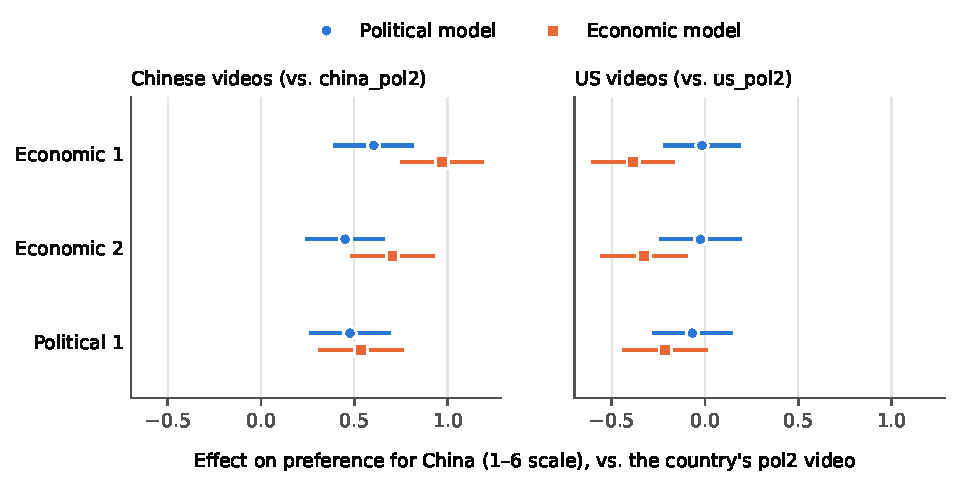
\includegraphics[width=\linewidth]{fig3_competition_videos.pdf}
\caption{Effect of each video relative to its country's \vid{pol2} video in the Competition arm. Chinese-video estimates control for the US video and vice versa. Lines are unadjusted 95\% confidence intervals.}
\label{fig:videos}
\end{figure}

\subsection{Two Designs, One Pattern}

The single-country arms and the Competition arm are independent samples with different designs, so it is informative to compare them. The Competition estimates imply that, relative to \vid{china\_pol1}, the average CGTN economic video changes preference for China's political model by 0.05 points and its economic model by 0.30 points. The corresponding within-China-arm estimates are 0.01 and 0.26. For the US videos, the two designs agree on the political outcome (0.05 versus 0.08) but diverge somewhat on the economic outcome ($-0.14$ versus 0.01). Given standard errors of roughly 0.07 to 0.12, this gap could be noise, or US economic messages could matter more when they compete directly with Chinese ones. The data cannot distinguish between these explanations.

\section{Discussion}

The original study shows that Chinese state media can shift global opinion. The extension suggests that \emph{what} it says shapes how much opinion moves. Three conclusions follow.

First, content persuades mainly within its own domain. CGTN's economic videos raise preference for China's economic model but not, beyond a second political video, for its political model. This qualifies a natural reading of the performance-legitimacy argument, in which evidence of economic success should also make China's political system look more attractive. Among the respondents studied here, political and economic videos appear to be roughly interchangeable as arguments for the political model.

Second, individual messages differ substantially, and these differences are not explained by broad content categories. The most and least persuasive CGTN videos in the Competition arm differ by about 0.6 points on the political model and nearly 1 point on the economic model, comparable in size to the paper's main effects.

Third, these results bear on the interpretation of the headline estimate. Every respondent in the China arm saw \vid{china\_pol2}, which was the least persuasive CGTN video in the Competition arm. The China-arm effect is a valid estimate of the effect of the bundles that were actually shown. However, it may be conservative relative to other combinations of CGTN content. I emphasize that this is an inference across arms rather than a direct estimate: no respondent in the China arm saw a pair without \vid{china\_pol2}.

\paragraph{Limitations.} The extension relies on four videos per country. ``Economic'' and ``political'' videos also differ in length, style, and subject, so contrasts between types are best read as contrasts between these specific videos rather than between content categories in general. Within-arm subsamples are a quarter to a half the size of the arms, so the MDEs of 0.15 to 0.22 points mean that modest differences may go undetected, and the interaction estimates in the Competition arm are too imprecise to be informative. The replication package does not include the survey flow file, so the always-shown \vid{pol2} pattern is inferred from the data. Finally, the absence of a display-order variable rules out the order-effects analysis I originally planned.

\paragraph{Future directions.} The video-level variation documented here invites a direct study of message features. Researchers could code the videos for performance claims, explicit criticism of the United States, use of statistics, and production quality, and then randomize those features in a new experiment. Recovering the display order from the original survey platform would also make it possible to test whether the first or the last message has the advantage when Chinese and US narratives compete, a question with direct relevance to how international broadcasters compete for audiences.

\section*{Data and Code}

All code is available at \url{https://github.com/REPLACE-WITH-REPO-URL}. A single command (\texttt{python run\_all.py}) reproduces every table and figure from the authors' replication data (Harvard Dataverse, \url{https://doi.org/10.7910/DVN/CQ4FZR}).

\section*{References}

\begin{description}\setlength\itemsep{2pt}\small
\item Benjamini, Yoav, and Yosef Hochberg. 1995. ``Controlling the False Discovery Rate: A Practical and Powerful Approach to Multiple Testing.'' \emph{Journal of the Royal Statistical Society: Series B} 57(1): 289--300.
\item Holm, Sture. 1979. ``A Simple Sequentially Rejective Multiple Test Procedure.'' \emph{Scandinavian Journal of Statistics} 6(2): 65--70.
\item Mattingly, Daniel C., Trevor Incerti, Changwook Ju, Colin Moreshead, Seiki Tanaka, and Hikaru Yamagishi. 2025. ``Chinese State Media Persuades a Global Audience That the `China Model' Is Superior: Evidence from a 19-Country Experiment.'' \emph{American Journal of Political Science} 69(3): 1029--46. \url{https://doi.org/10.1111/ajps.12887}.
\item Samii, Cyrus, and Peter M.\ Aronow. 2012. ``On Equivalencies between Design-Based and Regression-Based Variance Estimators for Randomized Experiments.'' \emph{Statistics \& Probability Letters} 82(2): 365--70.
\end{description}

\appendix
\section*{Appendix}
\renewcommand{\thetable}{A\arabic{table}}
\setcounter{table}{0}

\begin{table}[ht]
\centering
\caption{Effect of each video relative to its country's \vid{pol2}, Competition arm}
\label{tab:videos}
\begin{tabular}{lcccccc}
\toprule
 & \multicolumn{3}{c}{Political model} & \multicolumn{3}{c}{Economic model} \\
\cmidrule(lr){2-4}\cmidrule(lr){5-7}
Video & Estimate (SE) & Holm $p$ & BH $p$ & Estimate (SE) & Holm $p$ & BH $p$ \\
\midrule
\vid{china\_econ1} & 0.605 (0.110) & $<$0.001 & $<$0.001 & 0.970 (0.115) & $<$0.001 & $<$0.001 \\
\vid{china\_econ2} & 0.451 (0.109) & $<$0.001 & $<$0.001 & 0.704 (0.114) & $<$0.001 & $<$0.001 \\
\vid{china\_pol1}  & 0.477 (0.110) & $<$0.001 & $<$0.001 & 0.536 (0.115) & $<$0.001 & $<$0.001 \\
\vid{us\_econ1}    & $-$0.015 (0.107) & 1.000 & 0.885 & $-$0.384 (0.114) & 0.004 & 0.001 \\
\vid{us\_econ2}    & $-$0.024 (0.113) & 1.000 & 0.885 & $-$0.326 (0.119) & 0.031 & 0.009 \\
\vid{us\_pol1}     & $-$0.067 (0.108) & 1.000 & 0.644 & $-$0.213 (0.116) & 0.262 & 0.087 \\
\midrule
$N$ & \multicolumn{3}{c}{1,459} & \multicolumn{3}{c}{1,456} \\
\bottomrule
\end{tabular}
\tablenote{\emph{Note:} One regression per outcome, including indicators for the Chinese video (reference \vid{china\_pol2}) and the US video (reference \vid{us\_pol2}), country fixed effects, covariates, and HC2 standard errors. $p$-values are adjusted across all twelve coefficients.}
\end{table}

\end{document}
